\section{Příklad 4}
% Jako parametr zadejte skupinu (A-H)
\ctvrtyZadani{D}

\section*{Riešenie}
\subsection*{1. krok}
Vyjadríme uhlovú frekvenciu:$$\omega = 2 \pi f = 2 \pi 85 = 170\pi \, rad/s$$\\
Prevedieme hodnoty na vyhovujúce jednotky:
\begin{equation*}
    \begin{aligned}
        L_1 = 180mH = 0,18H\\
        L_2 = 90mH = 0,09H
    \end{aligned}
    \qquad\qquad\qquad
    \begin{aligned}
        C_1 = 210\mu F = 210*10^{-6}F\\
        C_2 = 75\mu F = 75*10^{-6}F
    \end{aligned}
\end{equation*}\\
Vypočítame impedancie jednotlivých cievok a kondenzátorov:
\begin{equation*}
    \begin{aligned}
        Z_{L1} = i \omega L_1 \doteq 96,1327i \Omega\\\\
        Z_{L2} = i \omega L_2 \doteq 48,0664i \Omega
    \end{aligned}
    \qquad\qquad\qquad
    \begin{aligned}
        Z_{C1} = -\frac{i}{\omega c_1 }\doteq -8,9162i \Omega\\
        Z_{C2} = -\frac{i}{\omega c_2} \doteq -24,9655i \Omega
    \end{aligned}
\end{equation*}

\newpage
\subsection*{2. krok}
Zostavíme rovnice pre jednotlivé slučky.
\begin{center}
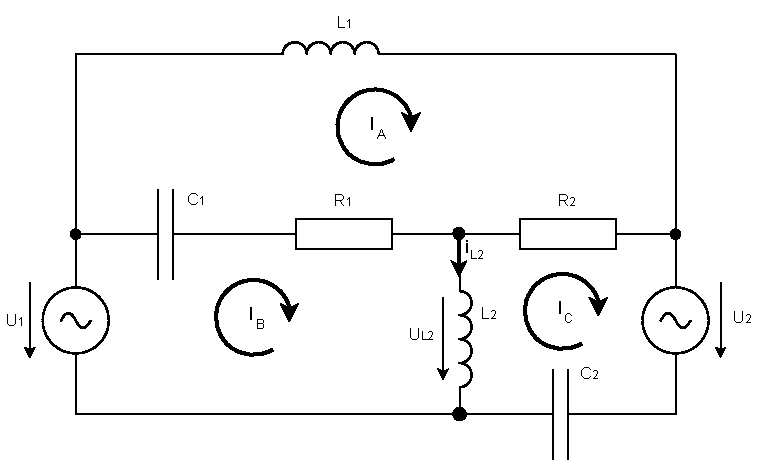
\includegraphics[scale=0.85,keepaspectratio]{xbednar00/zdroje/pr4/pr4_krok1.pdf}\\
\end{center}
$$I_A:I_A(Z_{L_1}+R_1+R_2+Z_{C_1})+I_B(-Z_{C_1}-R_1)+I_C(-R_2)=0$$
$$I_B:I_A(-Z_{C_1}-R_1)+I_B(Z_{C_1}+R_1+Z_{L_2})+I_C(-Z_{L_2})=u_1$$
$$I_C:I_A(-R_2)+I_B(-Z_{L_2})+U_C(R_2+Z_{C_2}+Z_{L_2})=-u_2$$\\
Rovnice prevedieme na maticový tvar.\\
$$\begin{pmatrix}
    Z_{L_1}+R_1+R_2+Z_{C_1} & -Z_{C_1}-R_1 & -R_2\\
    -Z_{C_1}-R_1 & R_1+Z_{L_2}+Z_{C_1} & -Z_{L_2}\\
    -R_2 & -Z_{L_2} & R_2+Z_{C_2}+Z_{L_2}\\
\end{pmatrix}
\times
\begin{pmatrix}
    I_A\\
    I_B\\
    I_C\\
\end{pmatrix}
=
\begin{pmatrix}
    0\\
    u_1\\
    -u_2
\end{pmatrix}$$\\
Maticu vyriešime pomocou Cramerovho pravidla (s výpočtom determinantu Sarrusovým pravidlom).\\
Výsledné hodnoty prúdov:\\
    $$I_A \doteq -0,0119 + 0,0157iA$$
    $$I_B \doteq -0,0206 - 0,0837iA$$
    $$I_C \doteq -0,0458 + 0,0203iA$$\\
Vypočítame $\pmb{|U_{L_2}|}$ a $\pmb{\varphi_{L_2}}$.\\
    $$I_{L_2} = I_B - I_C \doteq 0,0253 - 0,1040iA$$
    $$u_{L2} = Z_{L_2}*I_{L_2} \doteq 4,9986 + 1,2141iV$$\\
    $$\pmb{U_{L_2}} = \sqrt{{Re}(u_{L_2})^2 + {Im}(u_{L_2})^2} \doteq \pmb{5,1439V}$$
    $$\pmb{\varphi_{L_2}} = arctan\left(\frac{imag(u_{L_2})}{real(u_{L_2})}\right) \doteq arctan\left(\frac{1,2141}{4,9986}\right) \doteq 13,6524^{\circ} = \pmb{13^{\circ}39'}$$
    



